\documentclass{standalone}
\usepackage{hsbcommon}
\begin{document}
    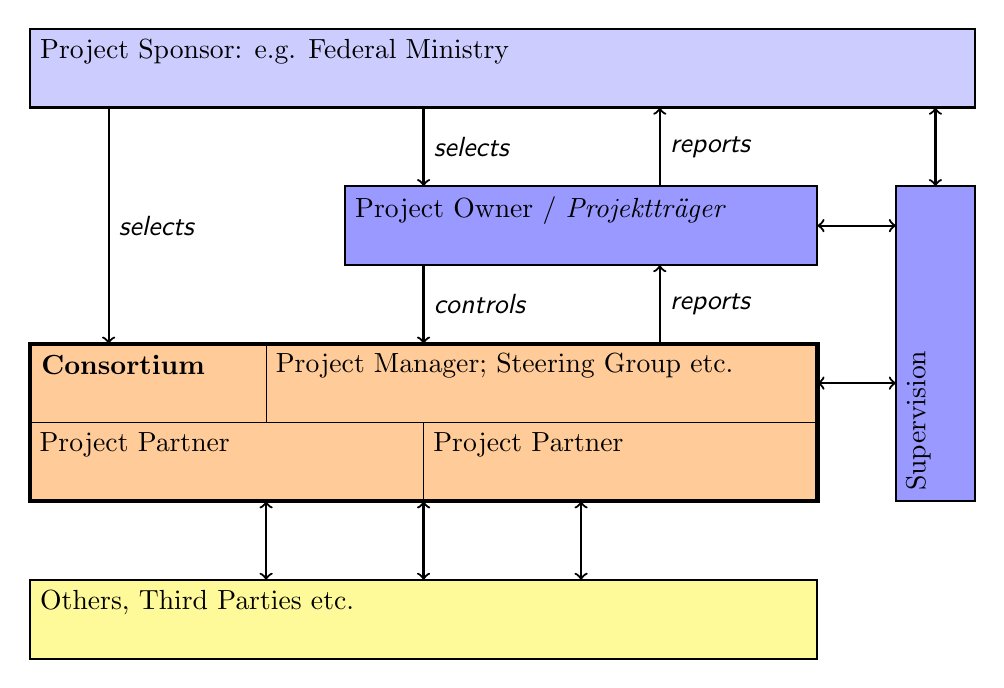
\begin{tikzpicture}
        \tikzset{action/.style={font=\itshape\sffamily}}
        \draw[thick,fill=blue!20]  (0,0) node[below right] {Project Sponsor: e.g. Federal Ministry} rectangle (12,-1);
        
        \draw[thick,->] (1,-1) -- node[right,action] {selects} (1,-4);
        \draw[thick,->] (5,-1) -- node[right,action] {selects} (5,-2);
        \draw[thick,<-] (8,-1) -- node[right,action] {reports} (8,-2);
        
        \draw[thick,<->] (11.5,-1) -- (11.5,-2);
        
        \draw[thick,fill=blue!40] (4,-2) node[below right] {Project Owner / \textit{Projektträger}} rectangle (10,-3);
        
        \draw[thick,->] (5,-3) -- node[right,action] {controls} (5,-4);
        \draw[thick,<-] (8,-3) -- node[right,action] {reports} (8,-4);
        
        \draw[thick,fill=blue!40] (11,-6) node[below right, rotate=90] {Supervision} rectangle (12,-2) ;
        
        \draw[thick,<->] (10,-2.5) -- (11,-2.5);
        \draw[thick,<->] (10,-4.5) -- (11,-4.5);

        \draw[thick,ultra thick,fill=orange!40] (0,-4) node[below right] {\textbf{Consortium}} rectangle (10,-6);

        \draw  (3,-4) node[below right] {Project Manager; Steering Group etc.} rectangle (10,-5);
        
        \draw (0,-5) node[below right] {Project
        Partner} rectangle (5,-6);
        
        \draw (5,-5) node[below right] {Project Partner} rectangle (10,-6);

        \draw[thick,<->] (3,-6) -- (3,-7);
        \draw[thick,<->] (5,-6) -- (5,-7);
        \draw[thick,<->] (7,-6) -- (7,-7);

        \draw[thick,fill=yellow!40] (0,-7) node[below right] {Others, Third Parties etc.} rectangle (10,-8);

    \end{tikzpicture}
\end{document}